\documentclass[UTF8]{ctexart}
\usepackage{bookmark}
\usepackage{geometry}
\usepackage{hyperref}
\geometry{a4paper,scale=0.8}
\usepackage{ctex}
\usepackage{booktabs}
\usepackage{array}
\usepackage{fancyhdr}
\usepackage{physics}
\pagestyle{fancy}
\fancyhf{}
\renewcommand\footrulewidth{1pt}
\lhead{\textit{王铠泽}}
\rhead{\textit{PB18020766}}
\chead{\href{mailto:volar@mail.ustc.edu.cn}{\textit{volar@mail.ustc.edu.cn}}}
\rfoot{\href{http://en.ustc.edu.cn/}{\textit{中国科学技术大学}}}
\lfoot{\textit{\today}}
\usepackage{graphicx}
\usepackage{float}
\usepackage{subfigure}
\fancyfoot[C]{\textit{\thepage}}


\begin{document}

	\centering\textbf{\LARGE{计算物理A第十七次作业}}
	
	
	王铠泽\qquad PB18020766
	
		
	\section{作业题目}
	
	\begin{itemize}
		\item 以$x_{n+1}=\lambda sin(\pi x_n)$为迭代方程进行迭代:
		
		\subitem (1) 画出系统状态随参数$\lambda$的变化图,要求在图中体现出定值状态、
		倍周期分叉和混沌状态;
		\subitem (2) 列出各个倍周期分叉处的$\lambda$值,求相应的 $Feigenbaum$ 常数。
	\end{itemize}
	
	
	\section{实现方法和原理}
	
	\begin{itemize}
		\item 稳态、倍周期分岔、混沌
		
		在动力系统迭代方程过程中,不同$\lambda$参数选择会导致系统最终处于不同的状态,比如稳态、周期态、混沌态(周期无穷)。下面是1维简单的$logistic$方程迭代的效果:
		
			\begin{figure}[H]
				\centering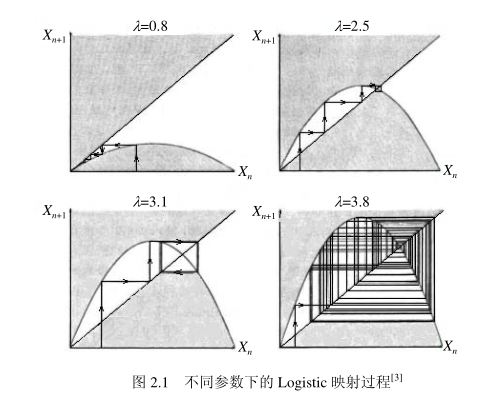
\includegraphics[width=4in]{eg}
				\end{figure}
		
			\begin{figure}[H]
			\centering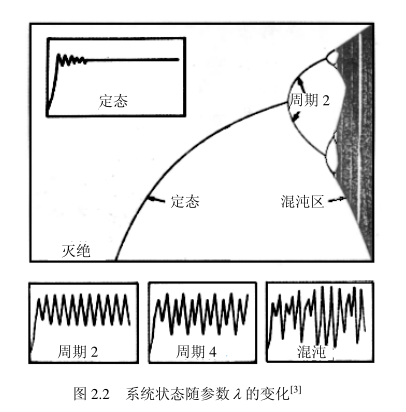
\includegraphics[width=2in]{x}
		\end{figure}
		\item $Feigenbaum$ 常数
		
		倍周期分岔处的$\lambda$值满足如下关系:
		
		$$\lim\limits_{m\rightarrow\infty}\frac{\lambda_m-\lambda_{m-1} }{\lambda_{m+1}-\lambda_{m}}=\delta(const)$$
		
		其中$\delta\approx4.669 201609102 990 671853 2038$,称为$Feigenbaum$ 常数。
		另一个简单的等价表述是:
		
		$$\lambda_{\infty}-\lambda_m=A\delta^{-m}(m\gg1)$$
		
		\item 摸拟实现
		
		本次摸拟算法很简单,直接利用迭代方程生成一组$\{x\}$序列。在一定的步长$M$之后取出若干$x$作为此时系统的状态点,观察稳态、周期态、混沌态的行为。
		
		关于$Feigenbaum$常数的计算,采用如下模式:
	
		本次实验关注从2周期分岔到128周期分岔的情况。使用一个长度为128数组$temp$来记录从$M$步之后的连续128个$x_k$的值,逐项和$temp[0]$比较,以$cnt$来记录周期计数,将每一个周期分岔处的$\lambda$值写入文件$Feigenbaum.txt$中。比较麻烦的是对于两个数是否相等的误差判定,随着周期增大,两个不同迭代点之间越来越接近,这使得计算误差和真正的周期性容易混淆,对于周期128的情况尤为明显。
	\end{itemize}
	
	\section{程式说明}
	
	\begin{itemize}
		\item chaos.c
		
		这是生成每一个$\lambda$对应系统最终状态的程式。将结果以文件的形式输出,$\lambda$范围和步长可以在程式中更改。
		
		\item Feigenbaum.c
		
		这是生成不同周期分岔处对应$\lambda$值的程式,结果以文件形式输出。计算$\lambda>0$和$\lambda<0$时步骤有少许不同,可在同一程式中更改(特别是两个数相等误差的判定有一些不同)。
		
		\item lambda(range).txt 
		
		这是不同$\lambda$范围和步长下的系统终态随$\lambda$变化的文件。
		
		\item Feigenbaum+/-.txt
		
		这分别对应$\lambda>0$和$\lambda<0$时周期分岔处的$\lambda$计算结果文件。
		
		\item 其他说明
		
		 本次程式中最终决定的总迭代步数为每个$x$迭代1000次,前100次舍去,$\lambda$的步进步长取其取值范围的$\frac{1}{1000000}$,运行时间可能较长,请耐心等待。或者自行改变步长。
	\end{itemize}
	
	\section{计算结果}
	
	\subsection{系统状态变化图}
	
	\begin{flushleft}
		选取不同的$\lambda$范围得到系统状态图,必要的时候缩小$\lambda$范围得到更精细的结构。
	\end{flushleft}
	
		\begin{figure}[H]
			\centering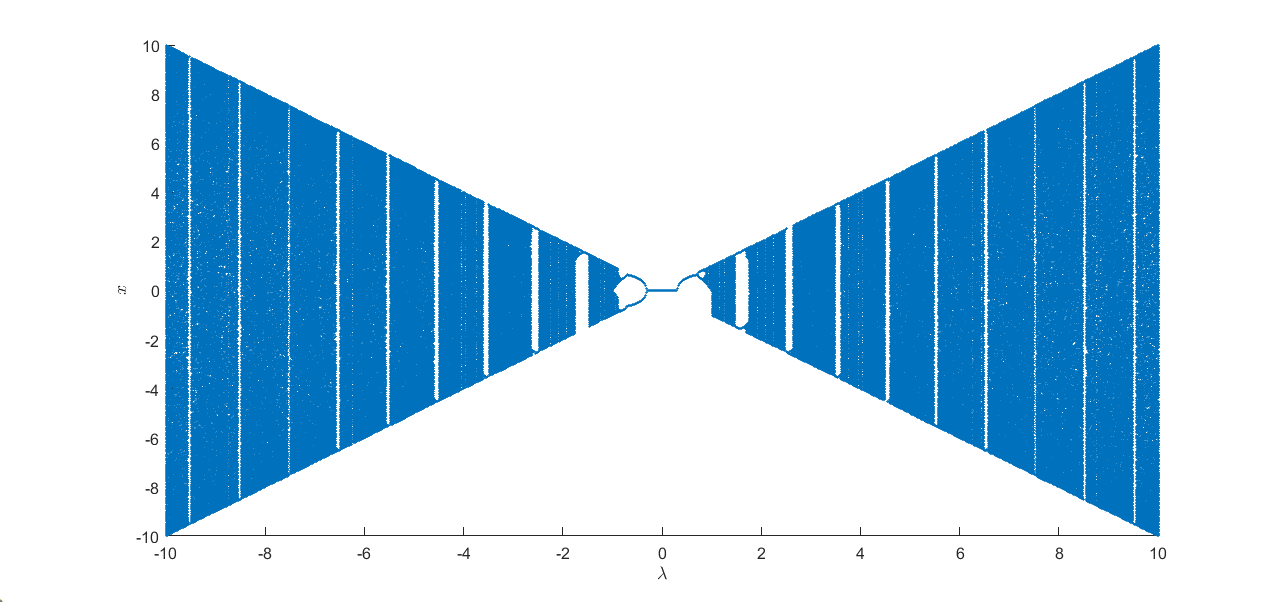
\includegraphics[width=6in]{../result/-10-10}
			\caption{$\lambda\in(-10,10)$}
			\end{figure}
	
\begin{flushleft}
		在比较大的尺度上,很明显地可以看到绝灭的稳态,呈现周期的态,以及大片大片的混沌态,还有混沌之中出现的周期窗口。
	
	有趣的是无论$\lambda>0$还是$\lambda<0$都能看到相似的现象,不同的仅在开始的时候正值$\lambda\approx1$处似乎缺了一块状态。下面给出几张更加精细的图片。
	
	
\end{flushleft}
	
\begin{figure}[H]
			\centering  %图片全局居中
			\subfigure[$\lambda\in(0,2.5)$]{
				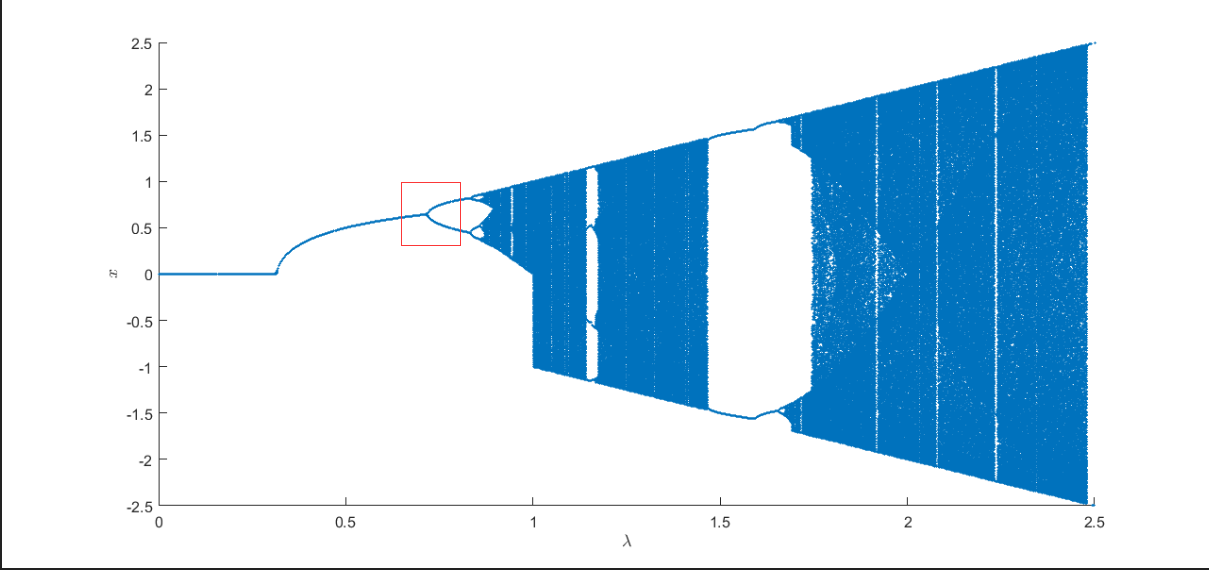
\includegraphics[width=0.45\textwidth]{../result/0-25.png}}
			\subfigure[$\lambda\in(0.8,0.95)$]{
				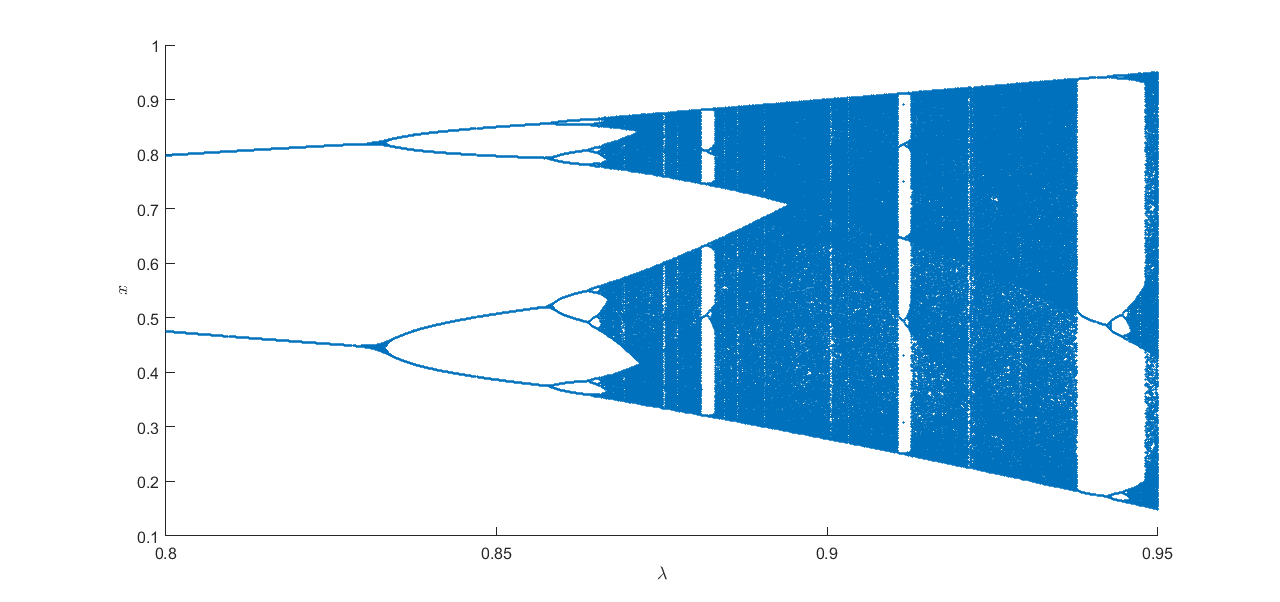
\includegraphics[width=0.45\textwidth]{../result/08-095}}
			\subfigure[$\lambda\in(0.86,0.88)$]{
				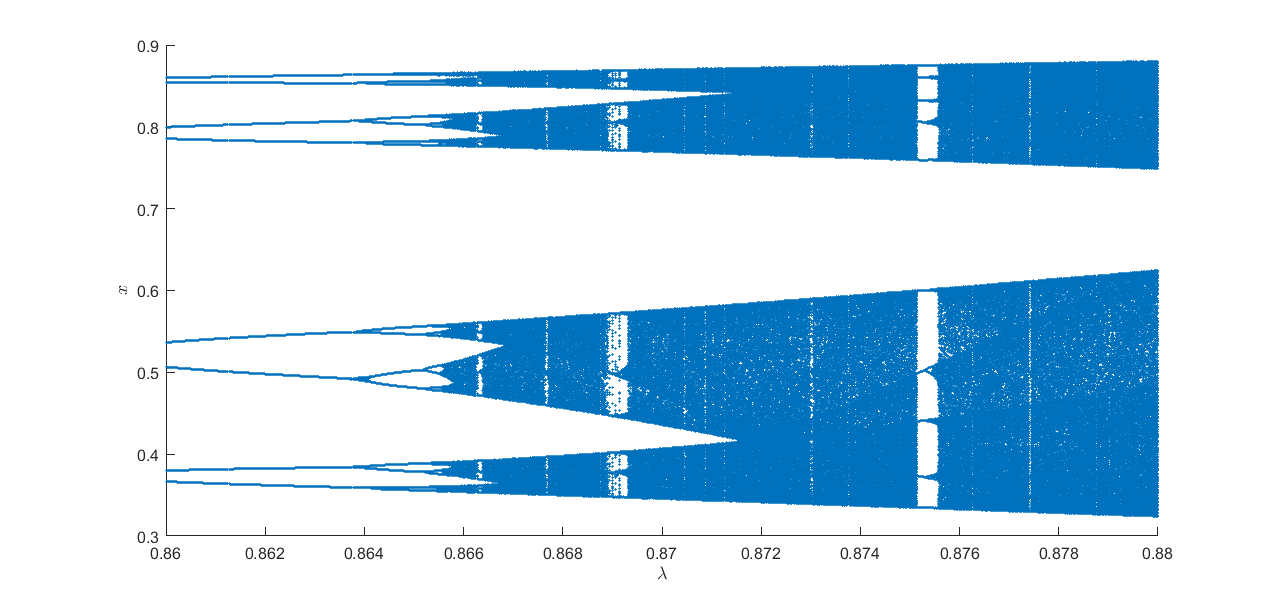
\includegraphics[width=0.45\textwidth]{../result/086-088}}
			\subfigure[$\lambda\in(0.714,0.726)$]{
				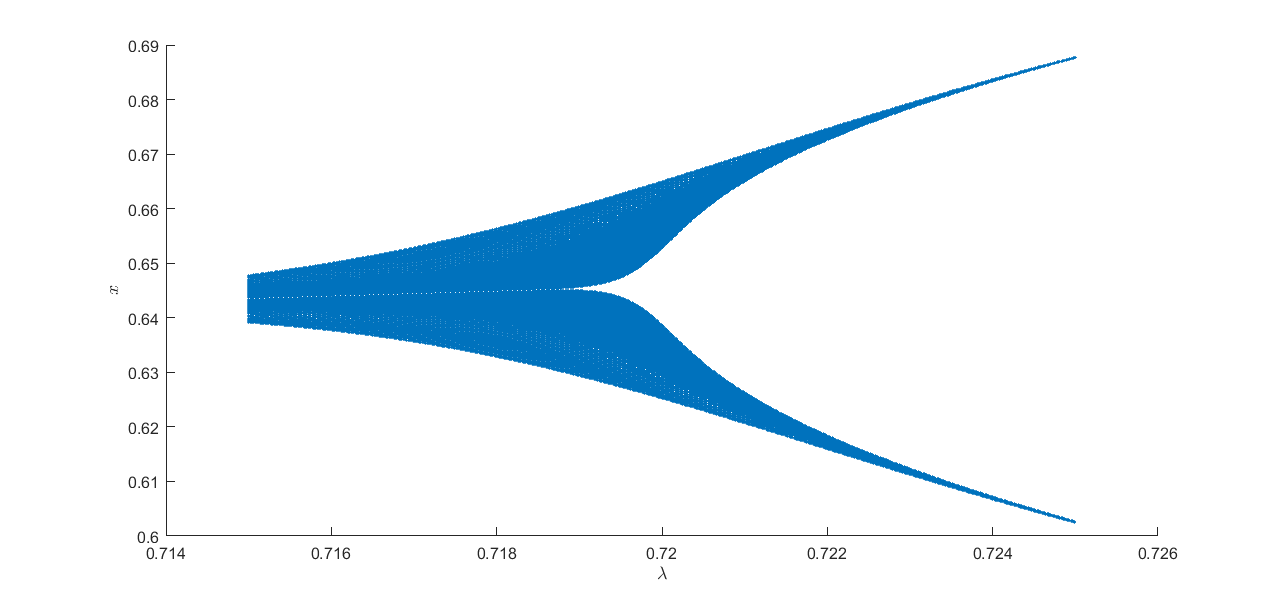
\includegraphics[width=0.45\textwidth]{../result/s}}
			\caption{不同范围下的图像$\lambda>0$}
	\end{figure}
	
	\begin{flushleft}
		值得注意的是(a)图中红框内部分放大后具有(d)图精细结构,不是简单的二值结构(这并非是计算误差导致的,(d)图已经将步长缩短10倍以上得到)。
	
	更好的说明上述现象,可以看下图的结构,将$0.8\sim0.95$的图放大:
	\end{flushleft}
	
	\begin{figure}[H]
		\centering  %图片全局居中
			\subfigure[$\lambda\in(0.8,0.95)$]{
			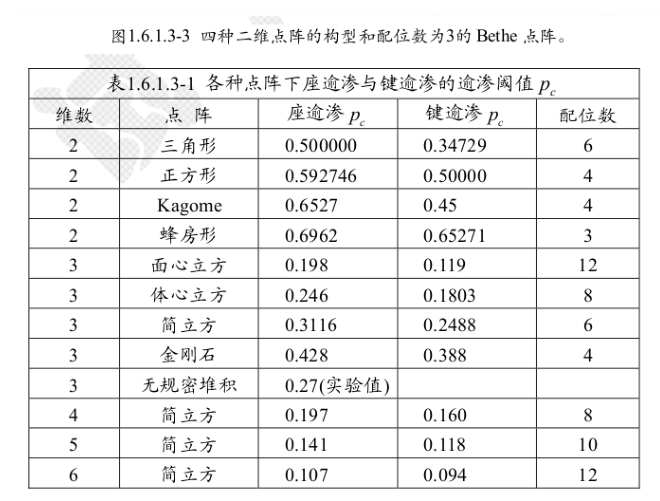
\includegraphics[width=0.45\textwidth]{../result/3}}
		\subfigure[红框]{
			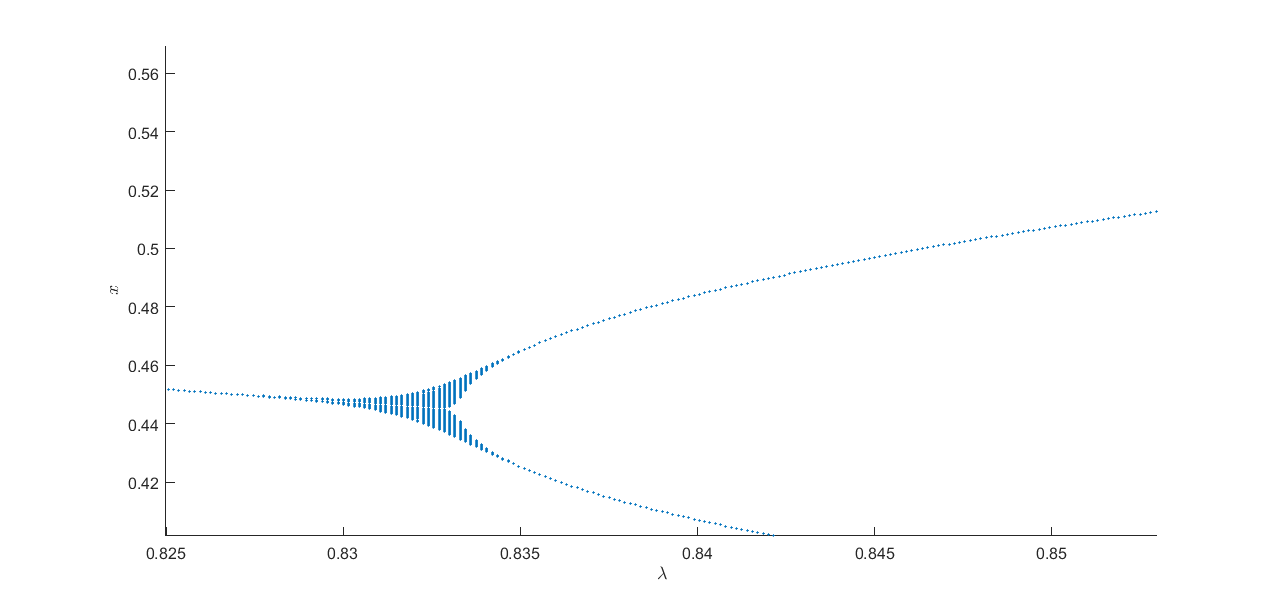
\includegraphics[width=0.45\textwidth]{../result/08-095_1}}
		\subfigure[放大]{
			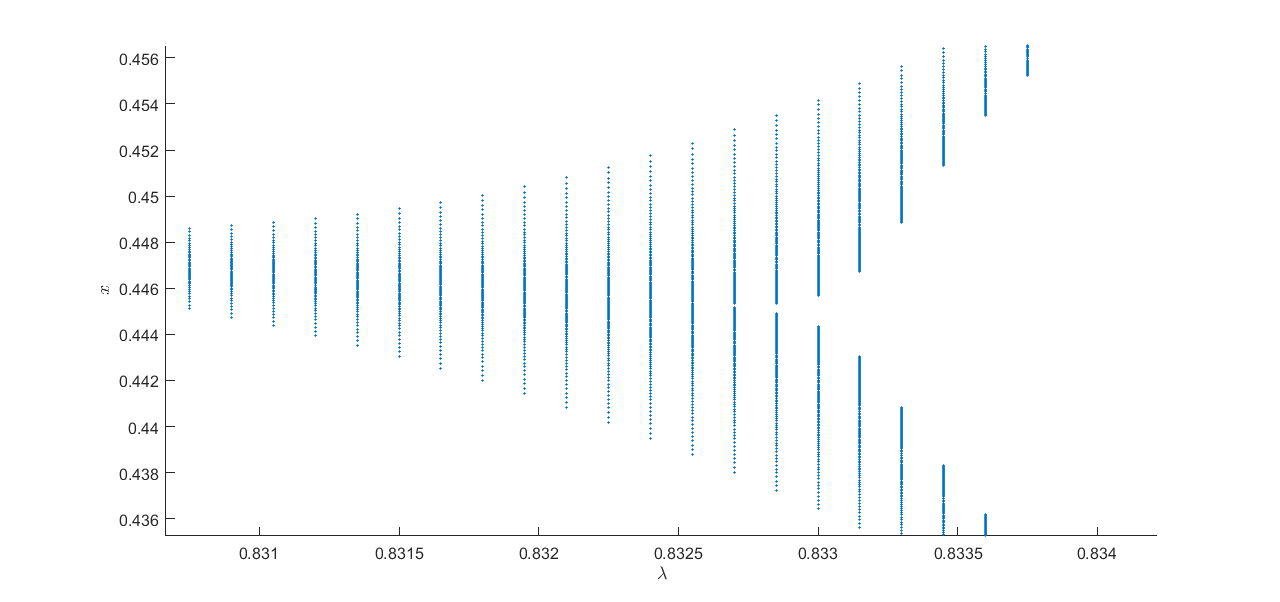
\includegraphics[width=0.45\textwidth]{../result/08-095_2}}
		\subfigure[再放大]{
			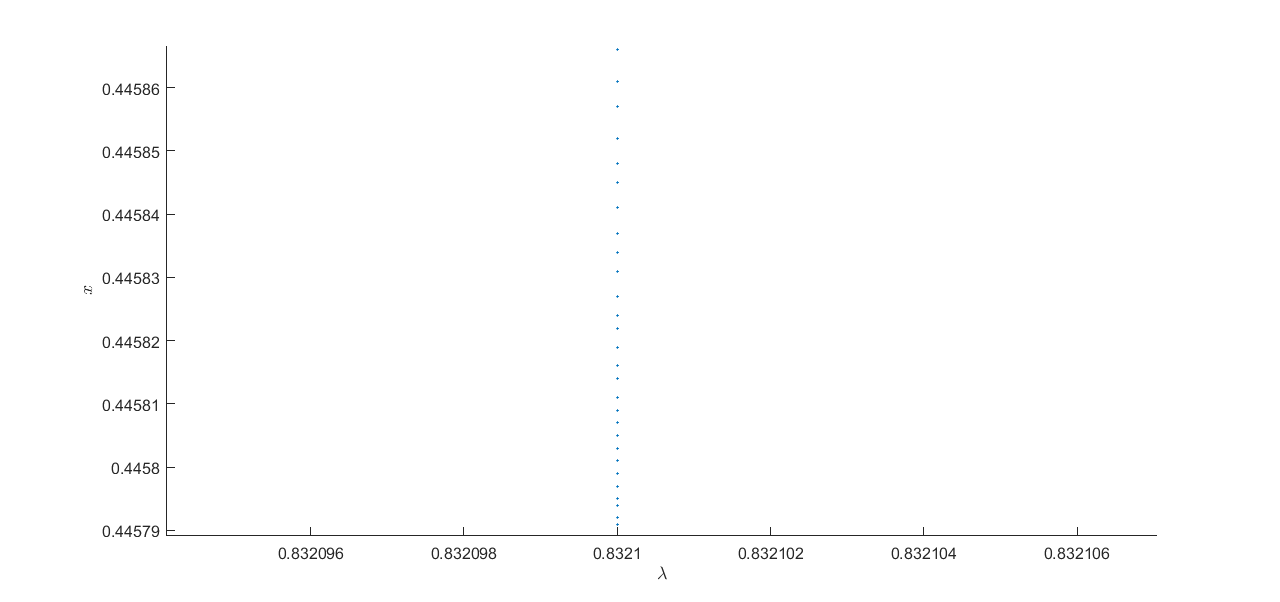
\includegraphics[width=0.45\textwidth]{../result/08-095_3.png}}
		\caption{分岔结构}
	\end{figure}
	
	\begin{flushleft}
		\textbf{可见这种分岔结构是一系列密集的点。}初步怀疑是计算精度的问题,但是仔细考虑这个分岔结构的宽度大概是有0.1的量级,不应该是由于计算误差导致的,可能是迭代方程本身带来的问题。
	\end{flushleft}
	
	\begin{flushleft}
		对于$\lambda<0$,同样可以给出不同范围的放大图像:
	\end{flushleft}
	
		\begin{figure}[H]
		\centering  %图片全局居中
		\subfigure[$\lambda\in(-1,1)$]{
			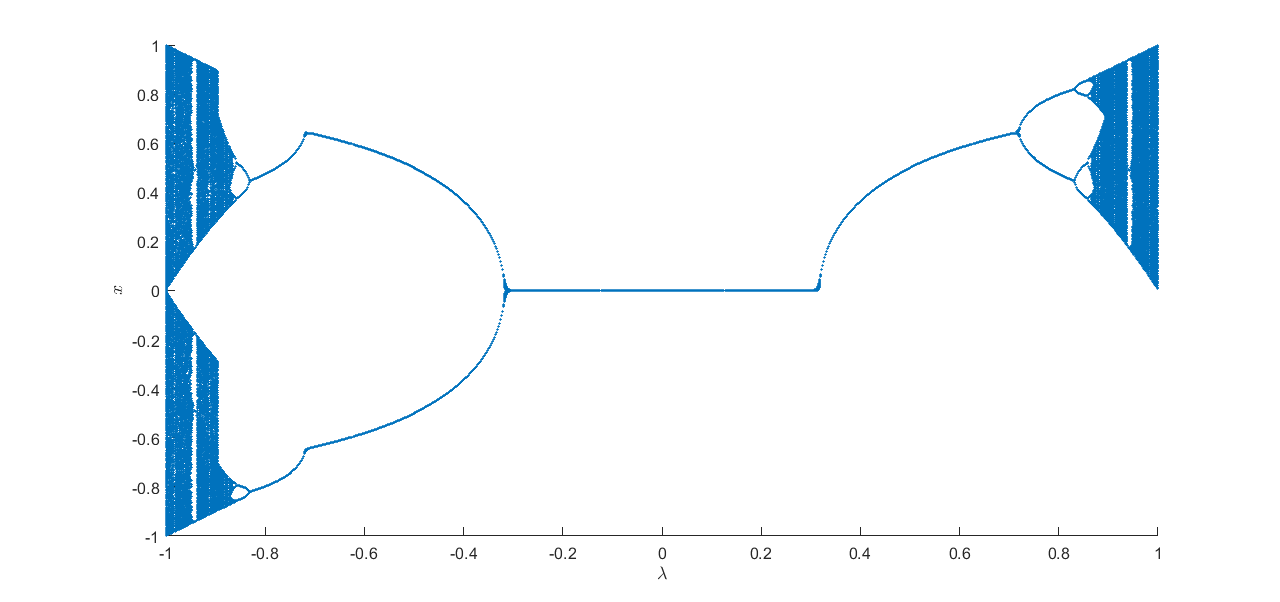
\includegraphics[width=0.45\textwidth]{../result/-1-1}}
		\subfigure[$\lambda\in(-1,-0.8)$]{
			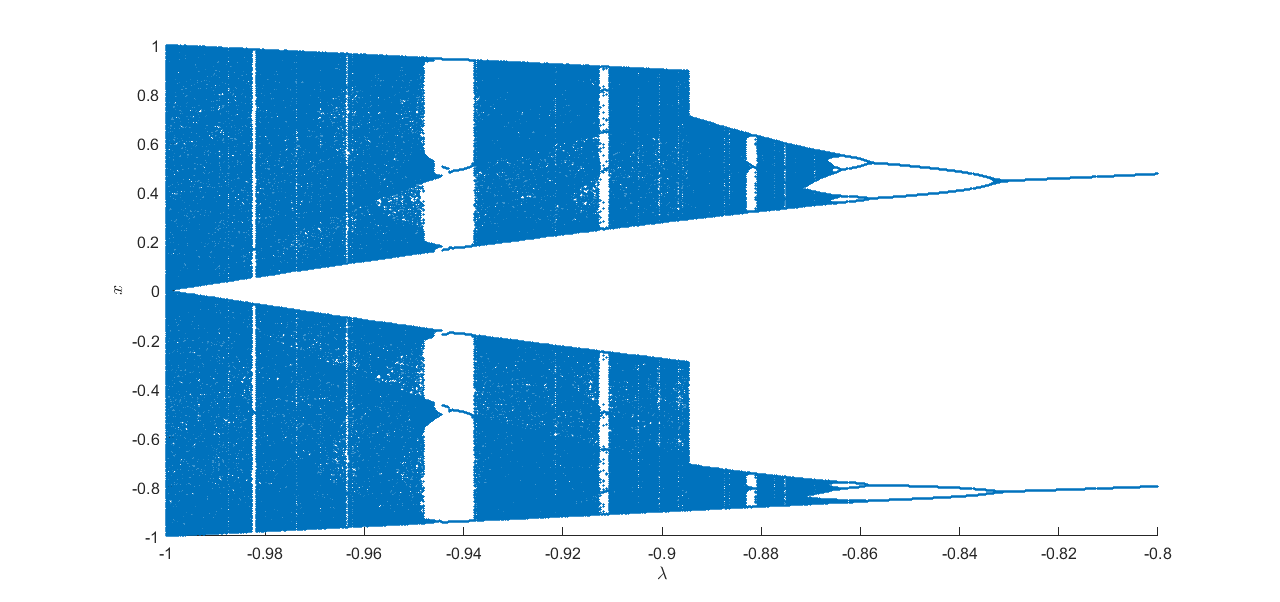
\includegraphics[width=0.45\textwidth]{../result/-1-08}}
		\caption{分岔结构}
	\end{figure}
	
	\subsection{$Feigenbaum$常数的计算}
	
	\begin{flushleft}
		根据程式得到结果列表如下:
	\end{flushleft}
	
	\setlength{\tabcolsep}{14mm}{
	\begin{table}[H]
		\centering
		\begin{tabular}{@{}ccc@{}}
			\toprule
			周期分岔&$\lambda_m$&$\frac{\lambda_m-\lambda_{m-1} }{\lambda_{m+1}-\lambda_{m}}$\\ \midrule
			1$\rightarrow$2	&0.7198504000&  \\
			2$\rightarrow$4&0.8338179200&4.5902\\
			4$\rightarrow$8	&0.8586462400&	4.4857	\\
			8$\rightarrow$16	&0.8641812800&	4.9941		\\
			16$\rightarrow$32	&0.8652896000&	4.7510	\\
			32$\rightarrow$64	&0.8655228800&  3.8984\\
			64$\rightarrow$128	&0.8655827200&	\\	\bottomrule
		\end{tabular}
	\caption{$\lambda>0$ case}
	\end{table}}
	
	\setlength{\tabcolsep}{14mm}{
		\begin{table}[H]
			\centering
			\begin{tabular}{@{}ccc@{}}
				\toprule
				周期分岔&$\lambda_m$&$\frac{\lambda_m-\lambda_{m-1} }{\lambda_{m+1}-\lambda_{m}}$\\ \midrule
				1$\rightarrow$2	&-0.3025601200&  \\
				2$\rightarrow$4&-0.8302080800&18.5542\\
				4$\rightarrow$8	&-0.8586462400&		5.1378\\
				8$\rightarrow$16	&-0.8641812800& 	4.9941		\\
				16$\rightarrow$32	&-0.8652896000&	4.7510\\
				32$\rightarrow$64	&-0.8655228800&	3.8984\\
				64$\rightarrow$128	&-0.8655827200&	\\	\bottomrule
			\end{tabular}
			\caption{$\lambda<0$ case}
	\end{table}}
	
	
	\begin{flushleft}
		\quad 可见$\lambda>0$和$\lambda<0$计算出来的$Feigenbaum$常数计算都不是非常准确(标为黑色加粗)。原因有很多,一个是之前提到的判定两数相等和周期分岔造成的麻烦,可以看到最后的$\lambda$相差应该只有$10^{-6}$量级。另一个是在初始多少步长才判定$x$迭代稳定,太小了不精确,太大了计算时间长,本实验采取1000作为初始步长。
	\end{flushleft}

\begin{flushleft}
		\quad 粗略地取平均值进行估计,$Feigenbaum$常数为$ 4.5439(\lambda>0)$和$4.6953(\lambda>0)$。和准确值$\delta$=4.669...仍有差距。并且我们能观察到其实算出来的$\Delta\lambda$比例对于$\lambda>0$和$\lambda<0$情况下出现很多一致,除了第一个点,这和我们之前对于图像的观察是一致的。两者的区别仅在于最开始缺了一块与否,这就是决定了第一个$\lambda$差别的地方,其他的值都是相反数,这从迭代方程就能很明显地看出,由于$sin$是奇函数,所以$\lambda$基本上不会改变迭代方程的性态。
\end{flushleft}


\begin{flushleft}
	接下来继续计算$\alpha$的值,根据定义:
\end{flushleft}

$$\alpha=\lim_{m\rightarrow\infty}\frac{d_{m}}{d_{m+1}}$$


	\begin{figure}[H]
	\centering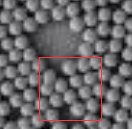
\includegraphics[width=4in]{../result/1}
	\caption{$Feigenbaum\,\,\alpha$}
	\end{figure}

\begin{flushleft}
	计算得到的分叉图片如下,选取纵坐标都为$0.5$:
\end{flushleft}

		\begin{figure}[H]
		\centering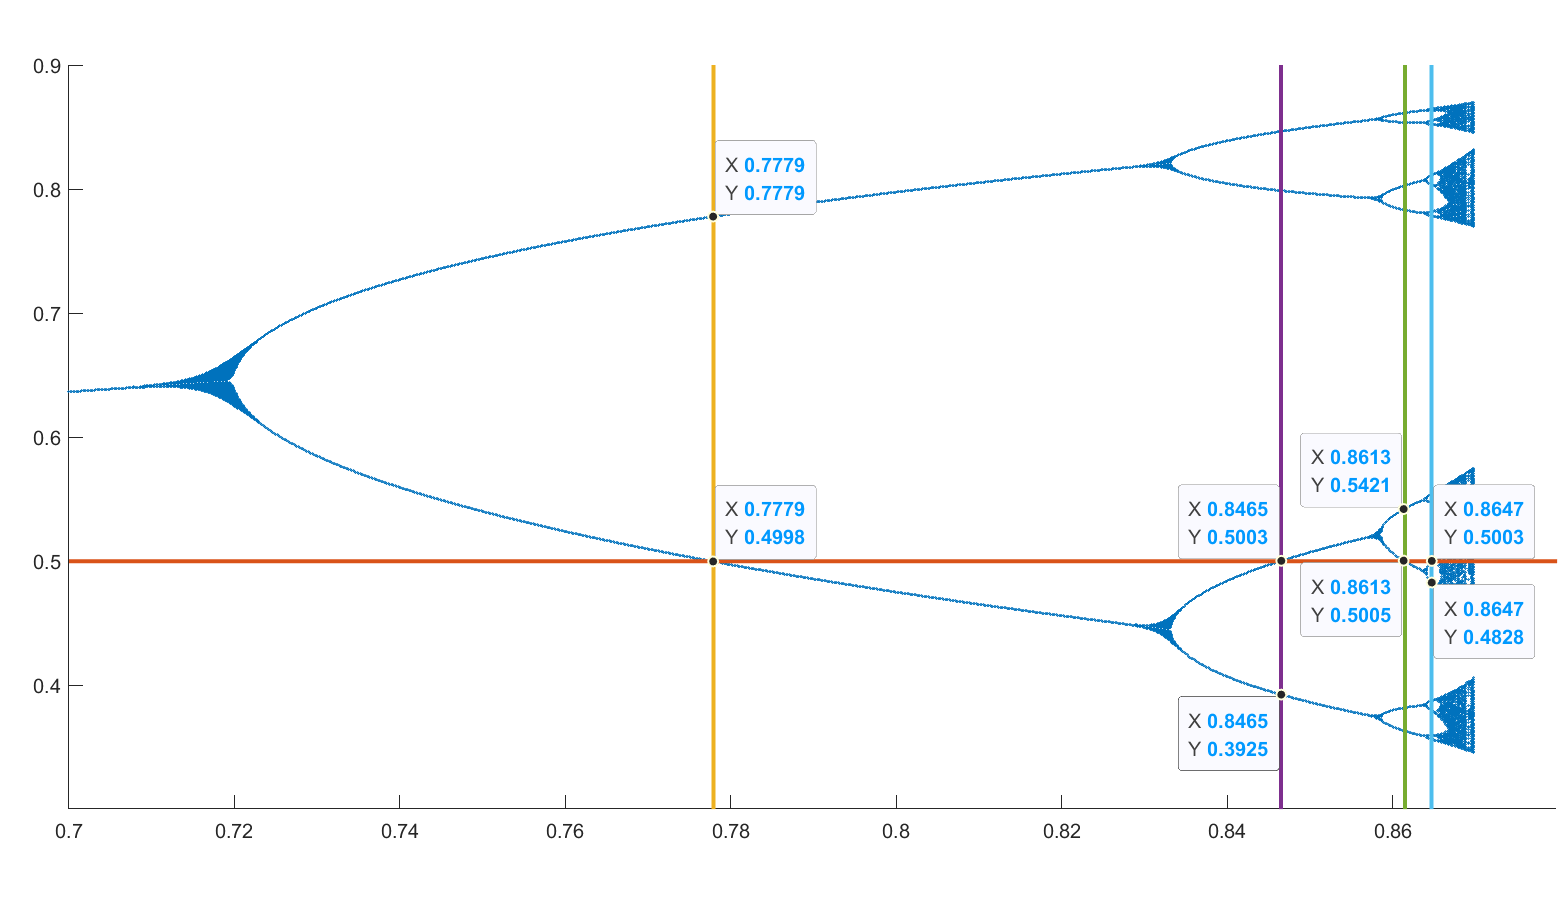
\includegraphics[width=6in]{../result/alpha}
		\caption{$Feigenbaum\,\,\alpha$}
	\end{figure}

	


	\setlength{\tabcolsep}{14mm}{
	\begin{table}[H]
		\centering
		\begin{tabular}{@{}ccc@{}}
			\toprule
		周期分岔&$d_m$&$\frac{d_m}{d_{m+1}}$\\ \midrule
		1$\rightarrow$2	&0.2781&  \\
		2$\rightarrow$4&0.1087&2.5584\\
		4$\rightarrow$8	&0.0416&2.6123\\
		8$\rightarrow$16&0.0175&2.3771\\ \bottomrule
		\end{tabular}
		\caption{$\lambda<0$ case}
\end{table}}

\begin{flushleft}
	$\alpha$计算值和准确值2.502有一定偏差,但仍算准确,可能的原因在于没有缩短$\lambda$步长,进行更为精确的计算。
\end{flushleft}

%	\begin{figure}[H]
%	\centering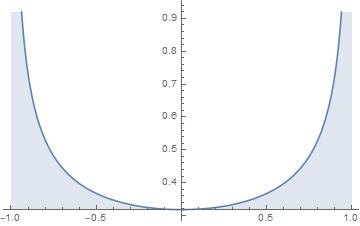
\includegraphics[width=2in]{1.jpg}
%	\caption{something}\label{fig:1}
%	\end{figure}
%		
%	\begin{figure}[H]
%		\centering  %图片全局居中
%		\subfigure[name1]{
%			\label{Fig.sub.1}
%			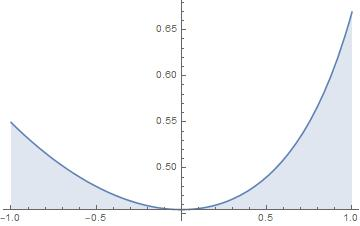
\includegraphics[width=0.45\textwidth]{2.jpg}}
%		\subfigure[name2]{
%			\label{Fig.sub.2}
%			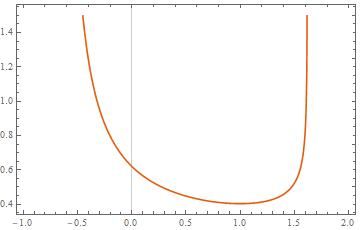
\includegraphics[width=0.45\textwidth]{3.jpg}}
%		\caption{Main name}
%		\label{Fig.main}
%	\end{figure}
	
	
	\section{总结}

	\begin{itemize}
		\item 迭代与混沌是物理中有趣的现象,本质上是微分方程的非线性性带来的效应。本次实验通过具体的模拟计算得到了从稳态向周期态和混沌态的过渡摸拟,计算了$Feigenbaum$常数,加深了对这一现象的理解。
		
	\end{itemize}

\end{document}